\documentclass[12pt,aspectratio=169]{beamer}
\usepackage{amsmath,amssymb,booktabs}
\usepackage{tikz,pgfplots}
\pgfplotsset{compat=1.18}
\usetikzlibrary{arrows.meta,positioning}

% ---- look of ch06v2 / ch07v2 ----
\setbeamertemplate{navigation symbols}{}
\definecolor{titlebg}{RGB}{214,214,240}
\definecolor{blocktitlebg}{RGB}{204,204,236}
\definecolor{blockbodybg}{RGB}{239,239,249}
\setbeamercolor{frametitle}{fg=black,bg=black!5}
\setbeamerfont{frametitle}{series=\bfseries,size=\large}
\setbeamercolor{title}{fg=black,bg=titlebg}
\setbeamerfont{title}{series=\bfseries,size=\LARGE}
\setbeamerfont{subtitle}{series=\bfseries,size=\large}
\setbeamercolor{block title}{fg=black,bg=blocktitlebg}
\setbeamercolor{block body}{fg=black,bg=blockbodybg}
\setbeamerfont{block title}{series=\bfseries}
\setbeamercolor{alerted text}{fg=red!80!black}
\setbeamertemplate{frametitle}{%
  \nointerlineskip
  \begin{beamercolorbox}[wd=\paperwidth,ht=2.6ex,dp=1.2ex,leftskip=.3cm]{frametitle}
    \usebeamerfont{frametitle}\insertframetitle
  \end{beamercolorbox}}
\setbeamertemplate{footline}{%
  \leavevmode\hbox to \paperwidth{\hskip.3cm
    {\tiny\color{black!55}\insertsectionhead\hfill\insertframenumber\,/\,\inserttotalframenumber}\hskip.3cm}
  \vskip2mm}
\setbeamertemplate{title page}{%
  \vfill
  \begin{beamercolorbox}[wd=\textwidth,sep=8pt,center]{title}
    {\usebeamerfont{title}\inserttitle\par}\vskip3pt
    {\usebeamerfont{subtitle}\insertsubtitle\par}
  \end{beamercolorbox}
  \vskip1.2em
  \begin{center}
    \insertauthor\par\vskip.8em
    {\small\insertinstitute}\par\vskip.8em
    \insertdate\par\vskip2em
    Reading: Nocedal \& Wright, \emph{Numerical Optimization}, 2nd ed., Chapter 5
  \end{center}
  \vfill}

\newcommand{\readpp}[1]{{\color{red!80!black}\textbf{Read:} #1}}
\newcommand{\eps}{\epsilon}
\newcommand{\R}{\mathbb{R}}
\newcommand{\xb}{\bar x}

\title{Advanced Optimization}
\subtitle{Chapter 5 --- Conjugate Gradient Methods}
\author{Hongseok Kim}
\institute{Department of Electronic Engineering, Sogang University}
\date{Fall 2026}

\newcommand{\algblock}[1]{\begin{block}{}#1\end{block}}
\newcommand{\kw}[1]{\textbf{#1}}
\newcommand{\ind}{\hspace*{1.2em}}
\newcommand{\K}{\mathcal{K}}

\begin{document}

\section{Chapter 5: introduction}

\begin{frame}
  \titlepage
\end{frame}

\begin{frame}{Conjugate gradient methods: two uses}
  \begin{columns}[T]
    \begin{column}{.48\textwidth}
      \begin{block}{Linear CG (\S5.1)}
        Hestenes and Stiefel, 1950s.
        Solves $Ax=b$, $A$ symmetric positive definite, without factorizing $A$.
        Speed depends on the \alert{eigenvalue distribution} of $A$; preconditioning improves it.
      \end{block}
    \end{column}
    \begin{column}{.48\textwidth}
      \begin{block}{Nonlinear CG (\S5.2)}
        Fletcher and Reeves, 1960s.
        One of the earliest large-scale methods.
        No matrix storage, faster than steepest descent.
      \end{block}
    \end{column}
  \end{columns}
  \vspace{1ex}
  Linear CG returns later in the course:
  \begin{itemize}
    \item Chapter 7: Newton--CG and CG--Steihaug (trust region).
    \item Chapter 16: projected CG for equality-constrained QP.
  \end{itemize}
  \readpp{pp.~101--102.}
\end{frame}

\section{\S5.1 Linear CG: conjugate directions}

\begin{frame}{One problem, two views}
  For $A\in\R^{n\times n}$ symmetric positive definite, these have the same unique solution $x^*$:
  \begin{equation}
    Ax=b \quad (5.1) \qquad\Longleftrightarrow\qquad
    \min_x\ \phi(x) \overset{\text{def}}{=} \tfrac12x^TAx-b^Tx. \tag{5.2}
  \end{equation}
  The gradient of $\phi$ is the residual of the linear system:
  \begin{equation}
    \nabla\phi(x) = Ax-b \overset{\text{def}}{=} r(x), \qquad r_k = Ax_k-b. \tag{5.3, 5.4}
  \end{equation}
  \begin{block}{Reading this chapter}
    ``Residual'' and ``gradient'' are the same thing.
    ``Minimize $\phi$ along $p$'' is an exact line search on a quadratic.
  \end{block}
\end{frame}

\begin{frame}{Conjugate directions}
  \begin{block}{Definition}
    Nonzero vectors $\{p_0,p_1,\dots,p_l\}$ are \textbf{conjugate} with respect to $A$ if
    \begin{equation}
      p_i^TAp_j = 0 \quad\text{for all } i\neq j. \tag{5.5}
    \end{equation}
  \end{block}
  A conjugate set is linearly independent (Exercise 5.2), so there are at most $n$ of them.

  \textbf{Conjugate direction method.} Given $x_0$ and conjugate $\{p_0,\dots,p_{n-1}\}$:
  \begin{equation}
    x_{k+1} = x_k+\alpha_kp_k, \qquad \alpha_k = -\frac{r_k^Tp_k}{p_k^TAp_k}. \tag{5.6, 5.7}
  \end{equation}
  $\alpha_k$ is the exact minimizer of $\phi$ along $x_k+\alpha p_k$ (see (3.55)).
\end{frame}

\begin{frame}{Theorem 5.1: at most $n$ steps}
  \begin{block}{Theorem 5.1}
    For any $x_0\in\R^n$, the sequence $\{x_k\}$ generated by (5.6), (5.7) converges to the solution $x^*$ of (5.1) in at most $n$ steps.
  \end{block}
  \textbf{Proof.} The $p_i$ span $\R^n$: $x^*-x_0=\sigma_0p_0+\cdots+\sigma_{n-1}p_{n-1}$.
  Multiply by $p_k^TA$; conjugacy leaves one term:
  \begin{equation}
    \sigma_k = \frac{p_k^TA(x^*-x_0)}{p_k^TAp_k}. \tag{5.8}
  \end{equation}
  Since $x_k = x_0+\alpha_0p_0+\cdots+\alpha_{k-1}p_{k-1}$, conjugacy gives $p_k^TA(x_k-x_0)=0$, so
  \[
    p_k^TA(x^*-x_0) = p_k^TA(x^*-x_k) = p_k^T(b-Ax_k) = -p_k^Tr_k.
  \]
  Compare with (5.7): $\sigma_k=\alpha_k$. \hfill$\square$
\end{frame}

\begin{frame}{The geometry}
  \begin{columns}[c]
    \begin{column}{.48\textwidth}
      \centering
      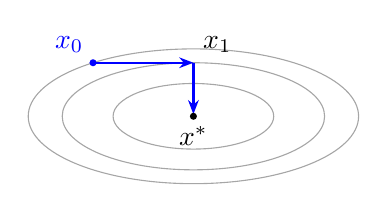
\begin{tikzpicture}[scale=0.85,>={Stealth[length=1.8mm]}]
        \foreach \ra/\rb in {2.468/1.007,1.960/0.800,1.2/0.49}
          \draw[black!35] (0,0) ellipse ({\ra} and {\rb});
        \draw[blue,thick,->] (-1.5,0.8)--(0,0.8);
        \draw[blue,thick,->] (0,0.8)--(0,0.03);
        \fill (0,0) circle (1.5pt) node[below] {$x^*$};
        \fill[blue] (-1.5,0.8) circle (1.5pt) node[above left] {$x_0$};
        \node[above right] at (0,0.8) {$x_1$};
      \end{tikzpicture}\\
      $A$ diagonal: done in $n$ steps (cf.\ Figure 5.1)
    \end{column}
    \begin{column}{.48\textwidth}
      \centering
      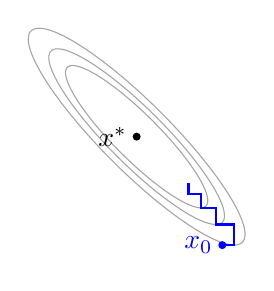
\begin{tikzpicture}[scale=1.45]
        \foreach \ra/\rb in {1.309/0.300,1.061/0.243,0.859/0.197}
          \draw[black!35] plot[domain=0:360,samples=72,smooth cycle] ({0.7071*(\ra*cos(\x)+\rb*sin(\x))},{0.7071*(-\ra*cos(\x)+\rb*sin(\x))});
        \draw[blue,thick]
          (0.750,-0.950)--(0.855,-0.950)--(0.855,-0.769)--(0.693,-0.769)--(0.693,-0.623)--(0.561,-0.623)
          --(0.561,-0.505)--(0.454,-0.505)--(0.454,-0.409);
        \fill (0,0) circle (1pt) node[left] {$x^*$};
        \fill[blue] (0.750,-0.950) circle (1pt) node[left] {$x_0$};
      \end{tikzpicture}\\
      General $A$: not finite (cf.\ Figure 5.2)
    \end{column}
  \end{columns}
  \vspace{1ex}
  \textbf{Fix: change variables.} With $S=[p_0\ p_1\cdots p_{n-1}]$ and $\hat x=S^{-1}x$ (5.9),
  $\hat\phi(\hat x)=\tfrac12\hat x^T(S^TAS)\hat x-(S^Tb)^T\hat x$, and $S^TAS$ is diagonal.
  Coordinate search in $\hat x$ is the conjugate direction method in $x$.
  \readpp{pp.~102--106.}
\end{frame}

\begin{frame}{Theorem 5.2: expanding subspace minimization}
  From (5.4) and (5.6): \ $r_{k+1} = r_k+\alpha_kAp_k$. \hfill (5.10)
  \begin{block}{Theorem 5.2 (Expanding Subspace Minimization)}
    For any $x_0$, the iterates of the conjugate direction method (5.6), (5.7) satisfy
    \begin{equation}
      r_k^Tp_i = 0, \quad i=0,1,\dots,k-1, \tag{5.11}
    \end{equation}
    and $x_k$ minimizes $\phi$ over the set
    \begin{equation}
      \{x \mid x=x_0+\mathrm{span}\{p_0,p_1,\dots,p_{k-1}\}\}. \tag{5.12}
    \end{equation}
  \end{block}
  After $k$ steps, $x_k$ is \alert{optimal on a $k$-dimensional subspace}: useful even when stopped early.
\end{frame}

\begin{frame}{Proof of Theorem 5.2}
  \textbf{Optimality.} Let $h(\sigma)=\phi(x_0+\sigma_0p_0+\cdots+\sigma_{k-1}p_{k-1})$, a strictly convex quadratic.
  Its minimizer satisfies $\partial h/\partial\sigma_i=0$, that is, $r(\tilde x)^Tp_i=0$ for $i<k$.
  So a point minimizes $\phi$ over (5.12) iff its residual is orthogonal to $p_0,\dots,p_{k-1}$.

  \vspace{1ex}
  \textbf{Induction on (5.11).} $k=1$: $x_1$ minimizes $\phi$ along $p_0$, so $r_1^Tp_0=0$.
  Assume $r_{k-1}^Tp_i=0$ for $i\le k-2$. By (5.10),
  \begin{align*}
    p_{k-1}^Tr_k &= p_{k-1}^Tr_{k-1}+\alpha_{k-1}p_{k-1}^TAp_{k-1} = 0 &&\text{by the choice (5.7) of } \alpha_{k-1},\\
    p_i^Tr_k &= p_i^Tr_{k-1}+\alpha_{k-1}p_i^TAp_{k-1} = 0, \ \ i\le k-2 &&\text{by hypothesis and conjugacy.}
  \end{align*}
  \hfill$\square$
\end{frame}

\section{\S5.1 Linear CG: the algorithm}

\begin{frame}{Generating the directions on the fly}
  Any conjugate set works: the eigenvectors of $A$, or Gram--Schmidt in the $A$-inner product.
  But eigenvectors cost too much, and Gram--Schmidt must store all previous directions.

  \textbf{CG}: use only the steepest descent direction $-r_k$ and the previous direction:
  \begin{equation}
    p_k = -r_k+\beta_kp_{k-1}. \tag{5.13}
  \end{equation}
  Require $p_{k-1}^TAp_k=0$:
  \[
    \beta_k = \frac{r_k^TAp_{k-1}}{p_{k-1}^TAp_{k-1}}.
  \]
  Start with $p_0=-r_0$, the steepest descent direction at $x_0$.
  \begin{block}{The surprise}
    We imposed conjugacy only with $p_{k-1}$, yet $p_k$ is conjugate to \emph{all} of $p_0,\dots,p_{k-1}$ (Theorem 5.3).
  \end{block}
\end{frame}

\begin{frame}{Algorithm 5.1 (CG, preliminary version)}
  \algblock{
    Given $x_0$; $r_0\leftarrow Ax_0-b$, $p_0\leftarrow-r_0$, $k\leftarrow0$;\\
    \kw{while} $r_k\neq0$\\
    \ind $\alpha_k\leftarrow -\dfrac{r_k^Tp_k}{p_k^TAp_k}$; \hfill (5.14a)\\[1ex]
    \ind $x_{k+1}\leftarrow x_k+\alpha_kp_k$; \hfill (5.14b)\\
    \ind $r_{k+1}\leftarrow Ax_{k+1}-b$; \hfill (5.14c)\\
    \ind $\beta_{k+1}\leftarrow \dfrac{r_{k+1}^TAp_k}{p_k^TAp_k}$; \hfill (5.14d)\\[1ex]
    \ind $p_{k+1}\leftarrow -r_{k+1}+\beta_{k+1}p_k$; \hfill (5.14e)\\
    \ind $k\leftarrow k+1$; \hfill (5.14f)\\
    \kw{end while}
  }
  Useful for proving properties. A cheaper version follows (Algorithm 5.2).
\end{frame}

\begin{frame}{Theorem 5.3: the four properties}
  Krylov subspace of degree $k$ for $r_0$:
  \begin{equation}
    \K(r_0;k) \overset{\text{def}}{=} \mathrm{span}\{r_0,Ar_0,\dots,A^kr_0\}. \tag{5.15}
  \end{equation}
  \begin{block}{Theorem 5.3}
    If the $k$th iterate of CG is not $x^*$, then
    \begin{align}
      r_k^Tr_i &= 0, \quad i=0,\dots,k-1, \tag{5.16}\\
      \mathrm{span}\{r_0,r_1,\dots,r_k\} &= \K(r_0;k), \tag{5.17}\\
      \mathrm{span}\{p_0,p_1,\dots,p_k\} &= \K(r_0;k), \tag{5.18}\\
      p_k^TAp_i &= 0, \quad i=0,\dots,k-1. \tag{5.19}
    \end{align}
    Therefore $\{x_k\}$ converges to $x^*$ in at most $n$ steps.
  \end{block}
\end{frame}

\begin{frame}{Proof of Theorem 5.3 (outline)}
  Induction on $k$ for (5.17)--(5.19).
  \begin{itemize}
    \item (5.17): $Ap_k\in\mathrm{span}\{Ar_0,\dots,A^{k+1}r_0\}$ (5.20), then (5.10) gives
      $r_{k+1}\in\K(r_0;k+1)$. Conversely $A^{k+1}r_0\in\mathrm{span}\{Ap_0,\dots,Ap_k\}$
      and $Ap_i=(r_{i+1}-r_i)/\alpha_i$.
    \item (5.18): by (5.14e), then (5.17).
    \item (5.19): multiply (5.14e) by $Ap_i$:
      \begin{equation}
        p_{k+1}^TAp_i = -r_{k+1}^TAp_i+\beta_{k+1}p_k^TAp_i. \tag{5.21}
      \end{equation}
      $i=k$: zero by the choice of $\beta_{k+1}$.
      $i<k$: Theorem 5.2 gives $r_{k+1}^Tp_j=0$, $j\le k$ (5.22), and $Ap_i\in\mathrm{span}\{p_0,\dots,p_{i+1}\}$ (5.23).
  \end{itemize}
  (5.16): $r_i\in\mathrm{span}\{p_i,p_{i-1}\}$, so (5.11) gives $r_k^Tr_i=0$.

  \alert{The proof needs $p_0=-r_0$.} With another $p_0$ the result fails.
  \readpp{pp.~107--111.}
\end{frame}

\begin{frame}{Remarks on Theorem 5.3}
  \begin{itemize}
    \item Residuals are mutually \textbf{orthogonal}; directions are mutually \textbf{conjugate}.
      ``Conjugate gradient'' is a misnomer: it is the directions, not the gradients, that are conjugate.
    \item CG is a \textbf{Krylov subspace method}: every iterate lies in $x_0+\K(r_0;k)$.
      This view gives the convergence rate.
    \item Only $p_{k-1}$ is needed to compute $p_k$: little storage and work.
  \end{itemize}
\end{frame}

\begin{frame}{Algorithm 5.2 (CG)}
  By (5.14e) and (5.11): $r_k^Tp_k=-r_k^Tr_k$. By (5.10) and (5.16): $\alpha_kr_{k+1}^TAp_k = r_{k+1}^Tr_{k+1}$. Hence
  \algblock{
    Given $x_0$; $r_0\leftarrow Ax_0-b$, $p_0\leftarrow-r_0$, $k\leftarrow0$;\\
    \kw{while} $r_k\neq0$\\
    \ind $\alpha_k\leftarrow\dfrac{r_k^Tr_k}{p_k^TAp_k}$; \quad
      $x_{k+1}\leftarrow x_k+\alpha_kp_k$; \quad
      $r_{k+1}\leftarrow r_k+\alpha_kAp_k$; \hfill (5.24a--c)\\[1ex]
    \ind $\beta_{k+1}\leftarrow\dfrac{r_{k+1}^Tr_{k+1}}{r_k^Tr_k}$; \quad
      $p_{k+1}\leftarrow-r_{k+1}+\beta_{k+1}p_k$; \quad $k\leftarrow k+1$; \hfill (5.24d--f)\\
    \kw{end while}
  }
  \readpp{pp.~111--112.}
\end{frame}

\begin{frame}{Algorithm 5.2: cost and use}
  \begin{itemize}
    \item Per iteration: one product $Ap_k$, two inner products $p_k^T(Ap_k)$ and $r_{k+1}^Tr_{k+1}$, three vector updates.
    \item Only $x$, $r$, $p$ from the last iteration are kept: overwrite in place.
    \item $A$ is never modified or factored: \alert{no fill-in}. $A$ can be given as a function $p\mapsto Ap$.
    \item For small $n$, use Gaussian elimination or another factorization: less sensitive to rounding.
      CG is recommended only for large problems.
    \item CG sometimes approaches the solution in far fewer than $n$ steps. Why? Next: the rate of convergence.
  \end{itemize}
\end{frame}

\section{\S5.1 Linear CG: rate of convergence}

\begin{frame}{The polynomial view}
  From (5.24b) and (5.18), for some polynomial $P_k^*$ of degree $k$:
  \begin{equation}
    x_{k+1} = x_0+\gamma_0r_0+\gamma_1Ar_0+\cdots+\gamma_kA^kr_0 = x_0+P_k^*(A)r_0. \tag{5.25, 5.26}
  \end{equation}
  With $\|z\|_A^2=z^TAz$ (5.27), the same norm as in Chapter 3,
  \begin{equation}
    \tfrac12\|x-x^*\|_A^2 = \phi(x)-\phi(x^*). \tag{5.28}
  \end{equation}
  By Theorem 5.2, $x_{k+1}$ minimizes $\phi$ over $x_0+\K(r_0;k)$. Hence
  \begin{equation}
    \|x_{k+1}-x^*\|_A = \min_{P_k}\ \|x_0+P_k(A)r_0-x^*\|_A. \tag{5.29}
  \end{equation}
  \alert{CG is optimal among all methods whose steps stay in the Krylov subspace.}
\end{frame}

\begin{frame}{Expanding in eigenvectors}
  $r_0=A(x_0-x^*)$, so $x_{k+1}-x^* = [I+P_k^*(A)A](x_0-x^*)$ (5.30).
  With eigenpairs $0<\lambda_1\le\cdots\le\lambda_n$, $v_i$, and $x_0-x^*=\sum_i\xi_iv_i$ (5.31):
  \begin{equation}
    \|x_{k+1}-x^*\|_A^2 = \sum_{i=1}^n\lambda_i[1+\lambda_iP_k^*(\lambda_i)]^2\xi_i^2. \tag{5.32}
  \end{equation}
  $P_k^*$ is optimal, so
  \begin{equation}
    \|x_{k+1}-x^*\|_A^2 \le \min_{P_k}\max_{1\le i\le n}[1+\lambda_iP_k(\lambda_i)]^2\ \|x_0-x^*\|_A^2. \tag{5.33}
  \end{equation}
  \begin{block}{The rate in one sentence}
    CG is as fast as a degree-$(k{+}1)$ polynomial $Q$ with $Q(0)=1$ can be made small on the eigenvalues of $A$.
    \alert{Where the eigenvalues are} matters, not $n$.
  \end{block}
\end{frame}

\begin{frame}{Theorem 5.4: distinct eigenvalues}
  \begin{block}{Theorem 5.4}
    If $A$ has only $r$ distinct eigenvalues, then CG terminates at the solution in at most $r$ iterations.
  \end{block}
  \textbf{Proof.} Let the distinct eigenvalues be $\tau_1<\cdots<\tau_r$ and
  \[
    Q_r(\lambda) = \frac{(-1)^r}{\tau_1\tau_2\cdots\tau_r}(\lambda-\tau_1)(\lambda-\tau_2)\cdots(\lambda-\tau_r).
  \]
  Then $Q_r(\lambda_i)=0$ for all $i$ and $Q_r(0)=1$, so $\bar P_{r-1}(\lambda)=(Q_r(\lambda)-1)/\lambda$ is a polynomial of degree $r-1$.
  In (5.34) with $k=r-1$:
  \[
    0 \le \min_{P_{r-1}}\max_i[1+\lambda_iP_{r-1}(\lambda_i)]^2 \le \max_iQ_r^2(\lambda_i) = 0.
  \]
  By (5.33), $x_r=x^*$. \hfill$\square$
\end{frame}

\begin{frame}{Theorem 5.5: clusters}
  \begin{block}{Theorem 5.5}
    If $A$ has eigenvalues $\lambda_1\le\lambda_2\le\cdots\le\lambda_n$, then
    \begin{equation}
      \|x_{k+1}-x^*\|_A^2 \le \left(\frac{\lambda_{n-k}-\lambda_1}{\lambda_{n-k}+\lambda_1}\right)^2\|x_0-x^*\|_A^2. \tag{5.35}
    \end{equation}
  \end{block}
  Idea: $Q_{k+1}$ with roots at the $k$ largest eigenvalues and at the midpoint of $[\lambda_1,\lambda_{n-k}]$.
  \vspace{.5ex}

  \begin{columns}[c]
    \begin{column}{.46\textwidth}
      \centering
      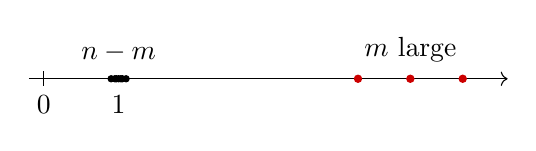
\begin{tikzpicture}[scale=0.95]
        \draw[->] (-0.2,0)--(6.2,0);
        \draw (0,0.1)--(0,-0.1) node[below] {0};
        \foreach \x in {0.9,0.95,1.0,1.05,1.1,0.97,1.03} \fill (\x,0) circle (1.4pt);
        \node[below] at (1,-0.1) {1};
        \foreach \x in {4.2,4.9,5.6} \fill[red!80!black] (\x,0) circle (1.6pt);
        \node[above] at (4.9,0.1) {$m$ large};
        \node[above] at (1,0.1) {$n-m$};
      \end{tikzpicture}\\
      cf.\ Figure 5.3
    \end{column}
    \begin{column}{.52\textwidth}
      $m$ large eigenvalues, the rest in a cluster of width $\epsilon$ near 1:
      after $m+1$ steps, $\|x_{m+1}-x^*\|_A\approx\epsilon\|x_0-x^*\|_A$.
    \end{column}
  \end{columns}
  More generally: $r$ clusters $\Rightarrow$ about $r$ iterations.
\end{frame}

\begin{frame}{Numerical example: clustered eigenvalues}
  \begin{columns}[T]
    \begin{column}{.56\textwidth}
      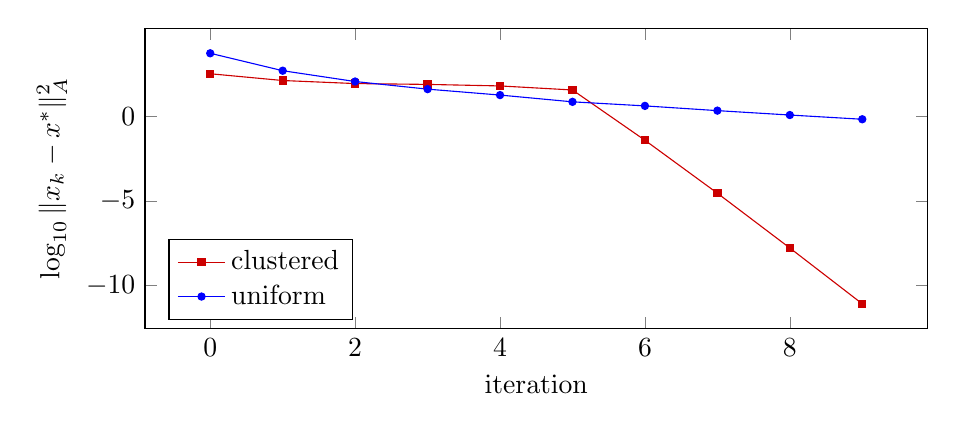
\begin{tikzpicture}
        \begin{axis}[width=.95\linewidth,height=5.4cm,
            xlabel={iteration},ylabel={$\log_{10}\|x_k-x^*\|_A^2$},
            xtick={0,2,4,6,8},ytick={-10,-5,0},
            legend style={at={(0.03,0.03)},anchor=south west},legend cell align=left]
          \addplot[red!80!black,mark=square*,mark size=1.3pt] coordinates {
            (0,2.53)(1,2.13)(2,1.95)(3,1.90)(4,1.81)(5,1.57)(6,-1.40)(7,-4.53)(8,-7.77)(9,-11.07)};
          \addplot[blue,mark=*,mark size=1.3pt] coordinates {
            (0,3.74)(1,2.71)(2,2.07)(3,1.62)(4,1.27)(5,0.87)(6,0.63)(7,0.35)(8,0.09)(9,-0.16)};
          \legend{clustered,uniform}
        \end{axis}
      \end{tikzpicture}
    \end{column}
    \begin{column}{.42\textwidth}
      $n=100$. (Not in the book; cf.\ Figure 5.4.)
      \begin{itemize}
        \item Clustered: 5 eigenvalues $20,\dots,100$, the other 95 in $[0.95,1.05]$.
          Sharp drop at iteration $6=m+1$, as Theorem 5.5 predicts.
        \item Uniform: eigenvalues spread over $[1,100]$.
          Slow, steady decrease.
      \end{itemize}
    \end{column}
  \end{columns}
\end{frame}

\begin{frame}{The condition-number bound}
  If only $\lambda_1$ and $\lambda_n$ are known, with $\kappa(A)=\lambda_n/\lambda_1$:
  \begin{equation}
    \|x_k-x^*\|_A \le 2\left(\frac{\sqrt{\kappa(A)}-1}{\sqrt{\kappa(A)}+1}\right)^k\|x_0-x^*\|_A. \tag{5.36}
  \end{equation}
  Steepest descent (3.29) has the same form with $\kappa$ in place of $\sqrt\kappa$.

  \vspace{1ex}
  \centering
  \renewcommand{\arraystretch}{1.1}
  \begin{tabular}{rcc}
    \toprule
    $\kappa$ & SD: iterations to reduce error by $10^6$ & CG\\
    \midrule
    $10^2$ & $\approx 690$ & $\approx 70$\\
    $10^4$ & $\approx 69{,}000$ & $\approx 690$\\
    $10^6$ & $\approx 6.9\times10^6$ & $\approx 6{,}900$\\
    \bottomrule
  \end{tabular}

  \raggedright
  \vspace{1ex}
  (5.36) is often a large overestimate; the eigenvalue distribution (Theorem 5.5) tells more.
  \readpp{pp.~112--118.}
\end{frame}

\begin{frame}{Numerical example: CG in floating point}
  Exercise 5.1: Hilbert matrix $A_{ij}=1/(i+j-1)$, $b=(1,\dots,1)^T$, $x_0=0$,
  stop when $\|r_k\|\le10^{-6}\|b\|$.

  \vspace{1ex}
  \centering
  \renewcommand{\arraystretch}{1.1}
  \begin{tabular}{rrr}
    \toprule
    $n$ & $\kappa(A)$ & CG iterations\\
    \midrule
    5 & $4.8\times10^{5}$ & 6\\
    8 & $1.5\times10^{10}$ & 19\\
    12 & $1.8\times10^{16}$ & 37\\
    20 & $1.0\times10^{19}$ & 68\\
    \bottomrule
  \end{tabular}

  \raggedright
  \vspace{1ex}
  More than $n$ iterations: in floating point the directions lose conjugacy, and Theorem 5.1 no longer applies.
  CG then behaves as an iterative method, and the rate theory still describes it. (Not in the book.)
\end{frame}

\section{\S5.1 Linear CG: preconditioning}

\begin{frame}{Preconditioning}
  Change variables with a nonsingular $C$:
  \begin{equation}
    \hat x = Cx, \qquad
    \hat\phi(\hat x) = \tfrac12\hat x^T(C^{-T}AC^{-1})\hat x-(C^{-T}b)^T\hat x. \tag{5.37, 5.38}
  \end{equation}
  CG on $\hat\phi$ converges according to the eigenvalues of $C^{-T}AC^{-1}$, not of $A$.
  \begin{block}{Goal}
    Choose $C$ so that $C^{-T}AC^{-1}$ has a small condition number, or better, clustered eigenvalues.
  \end{block}
  The transformation is never carried out. Run CG in $\hat x$, translate back to $x$:
  only $M=C^TC$ (symmetric positive definite) appears, and only through solves $My=r$.
\end{frame}

\begin{frame}{Algorithm 5.3 (Preconditioned CG)}
  \algblock{
    Given $x_0$, preconditioner $M$; $r_0\leftarrow Ax_0-b$; solve $My_0=r_0$; $p_0\leftarrow-y_0$; $k\leftarrow0$;\\
    \kw{while} $r_k\neq0$\\
    \ind $\alpha_k\leftarrow\dfrac{r_k^Ty_k}{p_k^TAp_k}$; \quad
      $x_{k+1}\leftarrow x_k+\alpha_kp_k$; \quad
      $r_{k+1}\leftarrow r_k+\alpha_kAp_k$; \hfill (5.39a--c)\\[1ex]
    \ind solve $My_{k+1}=r_{k+1}$; \hfill (5.39d)\\
    \ind $\beta_{k+1}\leftarrow\dfrac{r_{k+1}^Ty_{k+1}}{r_k^Ty_k}$; \quad
      $p_{k+1}\leftarrow-y_{k+1}+\beta_{k+1}p_k$; \quad $k\leftarrow k+1$; \hfill (5.39e--g)\\
    \kw{end while}
  }
  \begin{itemize}
    \item $M=I$ gives Algorithm 5.2.
    \item Orthogonality (5.16) becomes $r_i^TM^{-1}r_j=0$ for $i\neq j$. \hfill (5.40)
    \item Extra cost: one solve with $M$ per iteration. It must be cheap.
  \end{itemize}
\end{frame}

\begin{frame}{Practical preconditioners}
  No single choice is best. Trade-off: effectiveness of $M$, cost of forming and storing $M$, cost of solving $My=r$.
  \begin{itemize}
    \item \textbf{Problem-specific}: for a PDE, $My=r$ can be a coarser discretization of the same problem.
      Knowing where $A$ comes from is the key.
    \item \textbf{General purpose}: SSOR, banded, and \textbf{incomplete Cholesky} (probably the most effective).
      Compute $\tilde L$ no denser than the lower triangle of $A$, $A\approx\tilde L\tilde L^T$, $C=\tilde L^T$:
      \[
        C^{-T}AC^{-1} = \tilde L^{-1}A\tilde L^{-T}\approx I.
      \]
      $My=r$ is two triangular solves, about the cost of one $Ap$.
    \item \textbf{Pitfalls}: $\tilde L\tilde L^T$ may not be positive definite (increase the diagonal);
      breakdown can occur (allow more fill, at higher cost).
  \end{itemize}
  \readpp{pp.~118--120.}
\end{frame}

\begin{frame}{Numerical example: incomplete Cholesky}
  2-D Poisson equation, 5-point stencil on a $60\times60$ grid ($n=3600$).
  Stop when $\|r_k\|\le10^{-8}\|b\|$. (Not in the book.)

  \vspace{1ex}
  \centering
  \renewcommand{\arraystretch}{1.1}
  \begin{tabular}{lrr}
    \toprule
    & condition number & iterations\\
    \midrule
    CG, $M=I$ & $\kappa(A)=1507$ & 112\\
    PCG, $M=\tilde L\tilde L^T$, IC(0) & $\kappa(\tilde L^{-1}A\tilde L^{-T})=134$ & 49\\
    \bottomrule
  \end{tabular}

  \raggedright
  \vspace{1ex}
  \begin{itemize}
    \item IC(0): $\tilde L$ has the sparsity pattern of the lower triangle of $A$; no fill-in.
    \item $\kappa$ drops by a factor 11, so $\sqrt\kappa$ by about 3.4. The iteration count drops by 2.3.
  \end{itemize}
\end{frame}

\section{\S5.2 Nonlinear CG}

\begin{frame}{Algorithm 5.4 (Fletcher--Reeves)}
  Two changes to Algorithm 5.2: a line search on $f$ replaces (5.24a); $\nabla f$ replaces $r$.
  \algblock{
    Given $x_0$; evaluate $f_0=f(x_0)$, $\nabla f_0$; $p_0\leftarrow-\nabla f_0$; $k\leftarrow0$;\\
    \kw{while} $\nabla f_k\neq0$\\
    \ind compute $\alpha_k$ by a line search; $x_{k+1}=x_k+\alpha_kp_k$; evaluate $\nabla f_{k+1}$;\\
    \ind $\beta_{k+1}^{\rm FR}\leftarrow\dfrac{\nabla f_{k+1}^T\nabla f_{k+1}}{\nabla f_k^T\nabla f_k}$; \hfill (5.41a)\\[1ex]
    \ind $p_{k+1}\leftarrow-\nabla f_{k+1}+\beta_{k+1}^{\rm FR}p_k$; \hfill (5.41b)\\
    \ind $k\leftarrow k+1$; \hfill (5.41c)\\
    \kw{end while}
  }
  \begin{itemize}
    \item Strongly convex quadratic + exact line search: this is Algorithm 5.2.
    \item Each iteration needs only $f$ and $\nabla f$. No matrices, a few vectors.
  \end{itemize}
\end{frame}

\begin{frame}{Is $p_k$ a descent direction?}
  Take the inner product of (5.41b) with $\nabla f_k$:
  \begin{equation}
    \nabla f_k^Tp_k = -\|\nabla f_k\|^2+\beta_k^{\rm FR}\nabla f_k^Tp_{k-1}. \tag{5.42}
  \end{equation}
  Exact line search: $\nabla f_k^Tp_{k-1}=0$, so descent. Inexact: $p_k$ may be an \alert{ascent direction}.
  \begin{block}{Strong Wolfe conditions with $c_2<\frac12$}
    \vspace{-3ex}
    \begin{align}
      f(x_k+\alpha_kp_k) &\le f(x_k)+c_1\alpha_k\nabla f_k^Tp_k, \tag{5.43a}\\
      |\nabla f(x_k+\alpha_kp_k)^Tp_k| &\le -c_2\nabla f_k^Tp_k, \tag{5.43b}
    \end{align}
    with $0<c_1<c_2<\tfrac12$, not $c_2<1$ as in (3.7). Then every $p_k$ is a descent direction (Lemma 5.6).
    \hfill\readpp{pp.~121--122.}
  \end{block}
\end{frame}

\begin{frame}{Polak--Ribi\`ere and variants}
  \begin{align}
    \beta_{k+1}^{\rm PR} &= \frac{\nabla f_{k+1}^T(\nabla f_{k+1}-\nabla f_k)}{\|\nabla f_k\|^2}, \tag{5.44}\\
    \beta_{k+1}^{+} &= \max\{\beta_{k+1}^{\rm PR},0\} \quad\text{(PR+)}, \tag{5.45}\\
    \beta_{k+1}^{\rm HS} &= \frac{\nabla f_{k+1}^T(\nabla f_{k+1}-\nabla f_k)}{(\nabla f_{k+1}-\nabla f_k)^Tp_k}. \tag{5.46}
  \end{align}
  \begin{itemize}
    \item All equal $\beta^{\rm FR}$ on a strongly convex quadratic with exact line search, since then $\nabla f_{k+1}^T\nabla f_k=0$ (5.16).
    \item PR: more robust and efficient in practice. But strong Wolfe does \emph{not} guarantee descent for PR.
    \item HS: $p_{k+1}^T\bar G_kp_k=0$ with the average Hessian $\bar G_k=\int_0^1\nabla^2f(x_k+\tau\alpha_kp_k)\,d\tau$,
      since $\nabla f_{k+1}=\nabla f_k+\alpha_k\bar G_kp_k$.
  \end{itemize}
\end{frame}

\begin{frame}{More choices of $\beta$}
  Global convergence holds for any $\beta_k$ with
  \begin{equation}
    |\beta_k|\le\beta_k^{\rm FR}, \quad k\ge2. \tag{5.47}
  \end{equation}
  \textbf{FR--PR}: PR clipped to $[-\beta_k^{\rm FR},\beta_k^{\rm FR}]$ \hfill (5.48)

  \vspace{1ex}
  Two recent choices, with $\hat y_k=\nabla f_{k+1}-\nabla f_k$:
  \begin{align}
    \beta_{k+1} &= \frac{\|\nabla f_{k+1}\|^2}{\hat y_k^Tp_k} \qquad\text{(Dai--Yuan)}, \tag{5.49}\\
    \beta_{k+1} &= \left(\hat y_k-2p_k\frac{\|\hat y_k\|^2}{\hat y_k^Tp_k}\right)^T\frac{\nabla f_{k+1}}{\hat y_k^Tp_k} \qquad\text{(Hager--Zhang)}. \tag{5.50}
  \end{align}
  Both give descent directions under the (ordinary) Wolfe conditions, and are competitive with PR.
  \readpp{pp.~122--124.}
\end{frame}

\begin{frame}{Quadratic termination and restarts}
  \begin{itemize}
    \item Line searches use quadratic or cubic interpolation (Chapter 3): on a quadratic, $\alpha_k$ is exact and the method is Algorithm 5.2.
    \item \textbf{Restart every $n$ steps} ($\beta_k=0$): $n$-step quadratic convergence,
      \begin{equation}
        \|x_{k+n}-x^*\| = O(\|x_k-x^*\|^2). \tag{5.51}
      \end{equation}
      Near $x^*$, $f$ is nearly quadratic; after a restart there, the method is nearly linear CG, which needs $p_0=-\nabla f$.
    \item But CG is for large $n$, and a solution is often found in fewer than $n$ steps. Restart instead when consecutive gradients are far from orthogonal:
      \begin{equation}
        \frac{|\nabla f_k^T\nabla f_{k-1}|}{\|\nabla f_k\|^2}\ge\nu, \qquad \nu\approx0.1. \tag{5.52}
      \end{equation}
    \item PR+ (5.45) is also a restart: $p_{k+1}=-\nabla f_{k+1}$ whenever $\beta^{\rm PR}<0$. This is rare.
  \end{itemize}
  \readpp{pp.~124--125.}
\end{frame}

\section{\S5.2 Nonlinear CG: convergence}

\begin{frame}{Lemma 5.6: FR gives descent directions}
  \begin{block}{Lemma 5.6}
    Suppose Algorithm 5.4 uses step lengths that satisfy the strong Wolfe conditions (5.43) with $0<c_2<\tfrac12$.
    Then every $p_k$ is a descent direction, and
    \begin{equation}
      -\frac{1}{1-c_2} \le \frac{\nabla f_k^Tp_k}{\|\nabla f_k\|^2} \le \frac{2c_2-1}{1-c_2}, \quad k=0,1,\dots \tag{5.53}
    \end{equation}
  \end{block}
  \textbf{Proof idea.} $t(\xi)=(2\xi-1)/(1-\xi)$ increases on $[0,\tfrac12]$ from $-1$ to $0$, so the right side is in $(-1,0)$ (5.54).
  Induction: by (5.41),
  \begin{equation}
    \frac{\nabla f_{k+1}^Tp_{k+1}}{\|\nabla f_{k+1}\|^2} = -1+\frac{\nabla f_{k+1}^Tp_k}{\|\nabla f_k\|^2}, \tag{5.55}
  \end{equation}
  and (5.43b) bounds the last term by $c_2|\nabla f_k^Tp_k|/\|\nabla f_k\|^2$. Apply (5.53) for $k$. \hfill$\square$
\end{frame}

\begin{frame}{Why FR can stall}
  With $\cos\theta_k = -\nabla f_k^Tp_k/(\|\nabla f_k\|\,\|p_k\|)$ (5.56), Lemma 5.6 gives
  \begin{equation}
    \frac{1-2c_2}{1-c_2}\frac{\|\nabla f_k\|}{\|p_k\|} \le \cos\theta_k \le \frac{1}{1-c_2}\frac{\|\nabla f_k\|}{\|p_k\|}. \tag{5.57}
  \end{equation}
  So $\cos\theta_k\approx0$ iff $\|\nabla f_k\|\ll\|p_k\|$: a bad direction, likely a tiny step, and $\nabla f_{k+1}\approx\nabla f_k$.
  \begin{columns}[T]
    \begin{column}{.48\textwidth}
      \begin{block}{FR}
        $\beta_{k+1}^{\rm FR}\approx1$ (5.58), so $p_{k+1}\approx p_k$.
        The bad direction is kept: a long run of useless steps.
      \end{block}
    \end{column}
    \begin{column}{.48\textwidth}
      \begin{block}{PR (also PR+, HS, FR--PR)}
        $\beta_{k+1}^{\rm PR}\approx0$, so $p_{k+1}\approx-\nabla f_{k+1}$.
        An automatic restart.
      \end{block}
    \end{column}
  \end{columns}
  \vspace{1ex}
  Example in [123], $n=100$: FR needs thousands of iterations, PR needs 37.
  \alert{Never run FR without restarts.}
  \readpp{pp.~125--127.}
\end{frame}

\begin{frame}{Global convergence with restarts}
  \begin{block}{Assumptions 5.1}
    (i) The level set $\mathcal L=\{x\mid f(x)\le f(x_0)\}$ is bounded.\\
    (ii) $f$ is Lipschitz continuously differentiable in an open neighborhood $\mathcal N$ of $\mathcal L$.
  \end{block}
  Then $\|\nabla f(x)\|\le\bar\gamma$ on $\mathcal L$ (5.59), and Zoutendijk (Theorem 3.2) gives
  \begin{equation}
    \sum_{k=0}^\infty\cos^2\theta_k\|\nabla f_k\|^2<\infty. \tag{5.60}
  \end{equation}
  At restart iterations $k_1,k_2,\dots$, $\cos\theta_k=1$, so $\sum_j\|\nabla f_{k_j}\|^2<\infty$ (5.61), and
  \begin{equation}
    \liminf_{k\to\infty}\|\nabla f_k\|=0 \tag{5.62}
  \end{equation}
  for every method in this chapter, restarted at least every $\bar n$ steps.
  The interesting case: \alert{no restarts}.
\end{frame}

\begin{frame}{Theorem 5.7: Fletcher--Reeves without restarts}
  \begin{block}{Theorem 5.7 (Al-Baali)}
    Under Assumptions 5.1, Algorithm 5.4 with strong Wolfe steps, $0<c_1<c_2<\tfrac12$, satisfies
    \begin{equation}
      \liminf_{k\to\infty}\|\nabla f_k\|=0. \tag{5.63}
    \end{equation}
  \end{block}
  \textbf{Proof idea.} Suppose $\|\nabla f_k\|\ge\gamma>0$ (5.64).
  \begin{itemize}
    \item (5.57) in (5.60): $\sum_k\|\nabla f_k\|^4/\|p_k\|^2<\infty$, so $\sum_k1/\|p_k\|^2<\infty$. \hfill (5.65), (5.70)
    \item From (5.41b), (5.43b), (5.53), with $c_3=(1+c_2)/(1-c_2)$:
      $\|p_k\|^2\le c_3\|\nabla f_k\|^4\sum_{j\le k}\|\nabla f_j\|^{-2}\le c_3\bar\gamma^4k/\gamma^2$. \hfill (5.67), (5.68)
    \item Then $\sum_k1/\|p_k\|^2\ge\gamma_4\sum_k1/k=\infty$. Contradiction. \hfill$\square$
  \end{itemize}
  Extends to any $|\beta_k|\le\beta_k^{\rm FR}$, hence to FR--PR.
\end{frame}

\begin{frame}{Theorem 5.8: Polak--Ribi\`ere can cycle}
  \begin{block}{Theorem 5.8 (Powell)}
    Consider the Polak--Ribi\`ere method (5.44) with an ideal line search (the first positive stationary point of $f(x_k+\alpha p_k)$).
    There exist a twice continuously differentiable $f:\R^3\to\R$ and a starting point $x_0$
    such that $\{\nabla f_k\}$ is bounded away from zero.
  \end{block}
  \begin{itemize}
    \item The method that works best in practice has the weakest theory.
    \item The proof needs consecutive directions that become almost opposite;
      with ideal line searches, this happens only if $\beta_k<0$.
      Hence \textbf{PR+}: reset $\beta_k$ to 0 when negative.
    \item PR+ with a slightly modified Wolfe line search: descent and global convergence.
    \item (5.49) and (5.50): global convergence with the standard Wolfe conditions.
  \end{itemize}
  \readpp{pp.~127--131.}
\end{frame}

\begin{frame}{Numerical performance}
  Strong Wolfe, $c_1=10^{-4}$, $c_2=0.1$, no restarts; stop at $\|\nabla f_k\|_\infty<10^{-5}(1+|f_k|)$.
  Entries: iterations / function--gradient evaluations.

  \vspace{1ex}
  \centering
  \renewcommand{\arraystretch}{1.08}
  \begin{tabular}{llrrr}
    \toprule
    & Problem, $n$ & FR & PR & PR+\\
    \midrule
    Table 5.1 & GENROS, 500 & $*$ & 1068/2151 & 1067/2149\\
    & XPOWSING, 1000 & 533/1102 & 212/473 & 97/229\\
    & TRIDIA1, 1000 & 264/531 & 262/527 & 262/527\\
    \midrule
    Our run & ext.\ Rosenbrock, 1000 & 68/222 & 24/105 & 21/99\\
    & TRIDIA, 1000 & 669/887 & 961/1628 & 961/1628\\
    \bottomrule
  \end{tabular}

  \raggedright
  \vspace{1ex}
  $*$: no convergence in 10{,}000 iterations. ``Our run'': SciPy's strong Wolfe search; not in the book.
  PR is usually better, but not always. Book's advice: PR, PR+, FR--PR, or (5.49), (5.50).
\end{frame}

\section{Chapter 5: summary}

\begin{frame}{Chapter 5 in one table}
  \centering
  \renewcommand{\arraystretch}{1.1}
  \begin{tabular}{lll}
    \toprule
    & Linear CG (\S5.1) & Nonlinear CG (\S5.2)\\
    \midrule
    Problem & $Ax=b$, $A\succ0$ & $\min f$\\
    Direction & $p_k=-r_k+\beta_kp_{k-1}$ & $p_k=-\nabla f_k+\beta_kp_{k-1}$\\
    Step & exact, $r_k^Tr_k/p_k^TAp_k$ & strong Wolfe, $c_2<\tfrac12$\\
    $\beta_k$ & $r_k^Tr_k/r_{k-1}^Tr_{k-1}$ & FR, PR, PR+, HS, \dots\\
    Key property & conjugacy, Krylov optimality & descent (Lemma 5.6)\\
    Termination & $\le n$; $\le r$ distinct eigenvalues & $\liminf\|\nabla f_k\|=0$ (FR)\\
    Rate & $\sqrt\kappa$; clusters & $n$-step quadratic with restarts\\
    Cost & one $Ap$ per iteration & $f$, $\nabla f$, line search\\
    Accelerator & preconditioning & restarts, choice of $\beta$\\
    \bottomrule
  \end{tabular}
\end{frame}

\begin{frame}{Three results to carry forward}
  \begin{enumerate}
    \item \textbf{Conjugacy decouples the problem.}
      In the basis $\{p_i\}$, an $n$-dimensional quadratic is $n$ one-dimensional problems (Theorems 5.1, 5.2).
    \item \textbf{Eigenvalues, not $n$, set the speed.}
      $r$ distinct eigenvalues or clusters: about $r$ iterations. Preconditioning changes the distribution.
    \item \textbf{CG is optimal on the Krylov subspace (5.29).}
      This is why it can be stopped early, as in Newton--CG and CG--Steihaug (Chapter 7).
  \end{enumerate}
  \vspace{1ex}
  For nonlinear CG: strong Wolfe with $c_2<\tfrac12$, and PR-type $\beta$ or restarts.
\end{frame}

\begin{frame}{Homework {\normalsize (problems 5--6 are not in the book)}}
  \begin{enumerate}
    \item Exercise 5.2: a conjugate set is linearly independent.
    \item Exercise 5.6: show that (5.24d) is equivalent to (5.14d).
    \item Exercise 5.9: derive Algorithm 5.3 from Algorithm 5.2 in the variables $\hat x$.
    \item Exercise 5.11: PR (5.44) and HS (5.46) reduce to FR on a quadratic with exact line searches.
    \item Build $A\in\R^{100\times100}$ with exactly 5 distinct eigenvalues. Run Algorithm 5.2 and confirm Theorem 5.4.
      Then spread each eigenvalue into a cluster of width $10^{-2}$ and repeat.
    \item Implement FR and PR+ with a strong Wolfe line search ($c_2=0.1$) on extended Rosenbrock, $n=100$.
      Plot $\cos\theta_k$ and $\beta_k$.
  \end{enumerate}
\end{frame}

\end{document}
